\subchapter{Board setup}{Objective: setup communication
with the board and configure the bootloader.}

After this lab, you will be able to:
\begin{itemize}
\item Access the board through its serial line.
\item Interact with the stock bootloader
\end{itemize}

\section{Getting familiar with the board}

Take some time to read about the board features and connectors:

\begin{itemize}
   \item If you have the original BeagleBone Black: \url{http://www.elinux.org/Beagleboard:BeagleBoneBlack}
   \item If you have the newer BeagleBone Black Wireless:
\url{https://beagleboard.org/black-wireless} in addition to the above URL. 
\end{itemize}

Don't hesitate to share your questions with the instructor.

\section{Download technical documentation}

We are going to download documents which we will need during our
practical labs.

The main document to download is the BeagleBone Black System Reference Manual found at
\url{https://github.com/CircuitCo/BeagleBone-Black/blob/master/BBB_SRM.pdf?raw=true}.

Even if you have the BeagleBoneBlack Wireless board, this is the
ultimate reference about the board, in particular for the pinout and
possible configurations of the P8 and P9 headers, and more generally
for most devices which are the same in both boards.
You don't have to start reading this document now but you will need it
during the practical labs.

\section{Setting up serial communication with the board}

The Beaglebone serial connector is exported on the 6 pins close to one
of the 48 pins headers. Using your special USB to Serial adaptor provided
by your instructor, connect the ground wire (blue) to the pin closest
to the power supply connector (let's call it pin 1), and the \code{TX} (red)
and \code{RX} (green) wires to the pins 4 (board \code{RX}) and
5 (board \code{TX})\footnote{See
\url{https://www.olimex.com/Products/Components/Cables/USB-Serial-Cable/USB-Serial-Cable-F/}
for details about the USB to Serial adaptor that we are using.}.

You always should make sure that you connect the \code{TX} pin of the cable
to the \code{RX} pin of the board, and vice versa, whatever the board and
cables that you use.

\begin{center}
\includegraphics[width=8cm]{common/beaglebone-black-serial-connection.jpg}
\end{center}

Once the USB to Serial connector is plugged in, a new serial port
should appear: \code{/dev/ttyUSB0}.  You can also see this device
appear by looking at the output of \code{dmesg}.

To communicate with the board through the serial port, install a
serial communication program, such as \code{picocom}:

\begin{verbatim}
sudo apt install picocom
\end{verbatim}

If you run \code{ls -l /dev/ttyUSB0}, you can also see that only
\code{root} and users belonging to the \code{dialout} group have
read and write access to this file. Therefore, you need to add your user
to the \code{dialout} group:

\begin{verbatim}
sudo adduser $USER dialout
\end{verbatim}

{\bf Important}: for the group change to be effective, in Ubuntu 18.04, you have to
{\em completely reboot} the system \footnote{As explained on
\url{https://askubuntu.com/questions/1045993/after-adding-a-group-logoutlogin-is-not-enough-in-18-04/}.}.
A workaround is to run \code{newgrp dialout}, but it is not global.
You have to run it in each terminal.

Now, you can run \code{picocom -b 115200 /dev/ttyUSB0}, to start serial
communication on \code{/dev/ttyUSB0}, with a baudrate of \code{115200}. If
you wish to exit \code{picocom}, press \code{[Ctrl][a]} followed by
\code{[Ctrl][x]}.

There should be nothing on the serial line so far, as the board is not
powered up yet.

It is now time to power up your board by plugging in the mini-USB
(BeagleBone Black case) or micro-USB (BeagleBone Black Wireless case)
cable supplied by your instructor (with your PC or a USB power supply at the
other end of the cable).

See what messages you get on the serial line. You should see U-boot
start on the serial line.

\section{Bootloader interaction}

Reset your board. Press the space bar in the \code{picocom} terminal
to stop the U-boot countdown. You should then see the U-Boot prompt:

\begin{verbatim}
=>
\end{verbatim}

You can now use U-Boot. Run the \code{help} command to see the available
commands.

Type the \code{help saveenv} command to make sure that the
\code{saveenv} command exists. We use it in these labs to
save your U-Boot environment settings to the boards' eMMC storage.
Some earlier versions do not support this.

If you don't have this command, it's probably because you are doing these labs on your own
(i.e. without participating to a Bootlin course), we ask you to install the U-Boot binary
that we compiled and tested. See instructions in
\url{https://raw.githubusercontent.com/bootlin/training-materials/master/lab-data/common/bootloader/beaglebone-black/README.txt}
for a simple way to do this.

To avoid trouble because of settings applied in previous practical labs,
we advise you to clear the U-Boot environment variables:

\begin{verbatim}
env default -f -a
saveenv
\end{verbatim}

We are now ready to compile and use our own bootloader, kernel and root
filesystem.

\section{Attach the LCD cape}

Switch off the board first, by pressing the \code{POWER} button until
all the LEDs go off\footnote{That's strongly recommended by the board
maker, to avoid hardware damage that can happen if the board is abruptly
switched off.}.

Now that we have successfully tested serial console, we are ready to
attach the LCD4 cape provided by your instructor.

Note that if you bought your own Beagle Bone Black board, you will have
to {\bf gently} bend the serial headers using pliers, otherwise the
serial cable won't fit between the board and the cape.

There are two ways to connect the cape headers to the Bone Black
headers, but only one actually fits, the \code{POWER} button of the cape
sliding right between the board's RJ45 connector and power barrel
connector:
\begin{center}
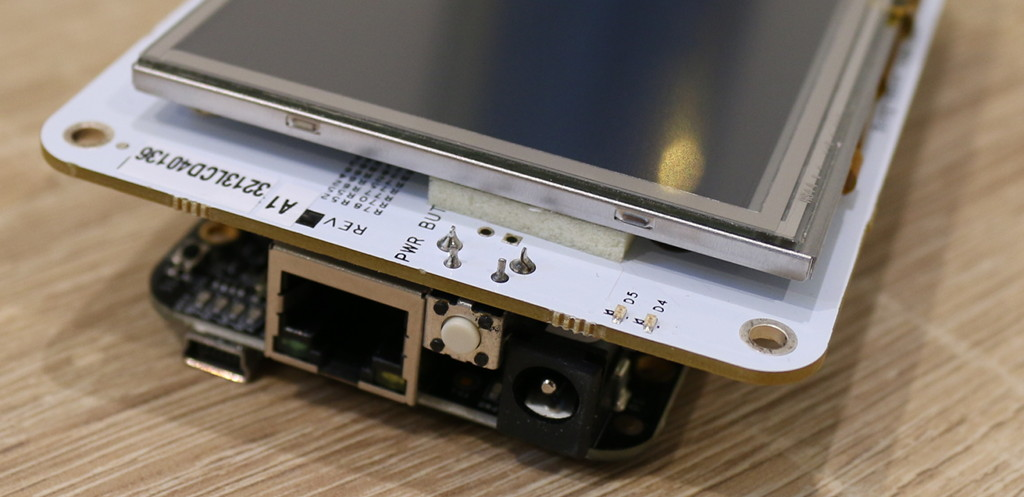
\includegraphics[width=8cm]{labs/boot-time-board-setup/connecting-lcd4-cape.jpg}
\end{center}

